% Section 4 draft: measuring whether joint reconciliation can help.
% Numbers marked \todo{} are filled from the pipeline results.

\section{Measuring whether joint reconciliation can help}
\label{sec:diagnostic}

Proposition~\ref{prop:equivalence} gives an exact condition, but in practice $\bm{W}$ is estimated and the condition never holds exactly in the estimate. We need a measure of how far an estimated covariance is from satisfying it, and a way to judge whether the observed departure is larger than estimation noise alone would produce.

\subsection{Separability is the wrong target}

The natural first choice is a measure of distance from a Kronecker product, such as the relative error of the nearest Kronecker approximation \citep{vanloan1993approximation}. Rearranging $\bm{W}$ so that each block $\bm{W}_{jk}$ becomes a row, $\bm{W}$ is a Kronecker product exactly when the rearranged matrix has rank one, and the relative error of the nearest Kronecker product is $\{1 - \sigma_1^2/\sum_i\sigma_i^2\}^{1/2}$, where $\sigma_i$ are its singular values. Likelihood ratio tests of separability are also available \citep{lu2005likelihood,mitchell2006likelihood}.

These measures answer the wrong question. By Corollary~\ref{cor:invariance}, reconciliation ignores any component of $\bm{W}$ of the form $\bm{S}_*\bm{K}\bm{S}_*'$, and such components can make $\bm{W}$ arbitrarily far from a Kronecker product without changing the reconciled forecasts at all. Conversely, departures that do change the forecasts may leave the Kronecker error small. Figure~\ref{fig:kronecker} plots the gain from joint reconciliation against the nearest-Kronecker error for the covariance families of Section~\ref{sec:simulation}. The Kronecker error rises with no gain at all when the departure is invisible, and it can fall while the gain rises.

\begin{figure}[!htb]
  \centering
  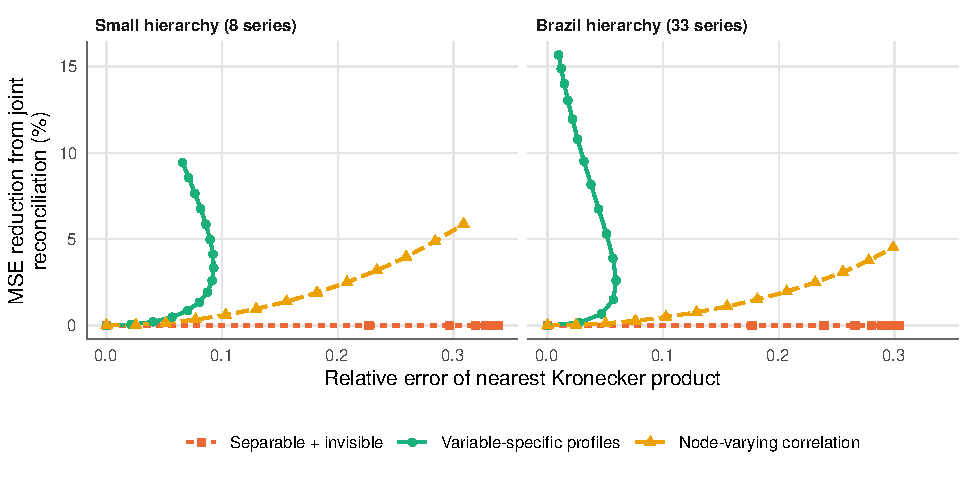
\includegraphics[width=\textwidth]{Imagens/kronecker_vs_gain.pdf}
  \caption{Population MSE reduction from joint reconciliation against the relative error of the nearest Kronecker approximation to $\bm{W}$, for the covariance families of Section~\ref{sec:simulation}.}
  \label{fig:kronecker}
\end{figure}

\subsection{Two measures}

We instead measure the conditions of Proposition~\ref{prop:equivalence} directly. The first measure describes the structure of the joint map. Since $\bm{G}$ contains the regression coefficients of the base forecast errors on the incoherences, and its off-diagonal blocks are the coefficients on other variables' incoherences, we define
\begin{equation}\label{eq:kappa}
  \kappa(\bm{W}) = \left(\frac{\sum_{j \ne k}\|\bm{G}_{jk}\|_F^2}{\|\bm{G}\|_F^2}\right)^{1/2},
\end{equation}
where $\bm{G}_{jk}$ is the $(n \times n_a)$ block of $\bm{G}$ relating the errors of variable $j$ to the incoherences of variable $k$. Rescaling variable $k$ by $c_k$ multiplies $\bm{G}_{jk}$ by $c_j/c_k$, so before computing $\kappa$ we standardise each variable by the square root of the mean diagonal of $\bm{W}_{jj}$. This makes $\kappa$ free of units. By Proposition~\ref{prop:equivalence}, $\kappa = 0$ exactly when joint and separate reconciliation coincide, and $\kappa$ inherits the invariance of Corollary~\ref{cor:invariance}.

The second measure describes the value of the joint map. If $\bm{W}$ were the true error covariance, the proportional reduction in mean squared error from reconciling jointly rather than separately would be
\begin{equation}\label{eq:gain}
  \gamma(\bm{W}) = 1 - \frac{\operatorname{tr}(\bm{M}\bm{W}\bm{M}')}{\operatorname{tr}(\bm{M}^{\mathrm{sep}}\bm{W}\bm{M}^{\mathrm{sep}\prime})}.
\end{equation}
MinT minimises the trace over all maps of this form, so $\gamma \ge 0$, again with equality exactly when the conditions of Proposition~\ref{prop:equivalence} hold. The two measures differ in an important way. The gain from any reconciliation comes only from the incoherent component of the errors, so $\gamma$ is small whenever that component is small, however strongly the joint map leans on other variables' incoherences. A large $\kappa$ with a small $\gamma$ says that joint reconciliation would change the forecasts but not improve them by much.

\subsection{Calibration}

Both measures are computed from an estimate $\widehat{\bm{W}}$, and both are biased in finite samples. Sampling noise pushes them above zero even when the population covariance satisfies Proposition~\ref{prop:equivalence}. The shrinkage estimator pulls the other way, because its diagonal target has no cross-variable blocks (Section~\ref{sec:theory}), so it shrinks genuine departures towards zero. Figure~\ref{fig:noise} shows both effects: \todo{describe noise floor and crossing, from exp1 results}. The raw values of $\kappa$ and $\gamma$ therefore cannot be read on an absolute scale.

\begin{figure}[!htb]
  \centering
  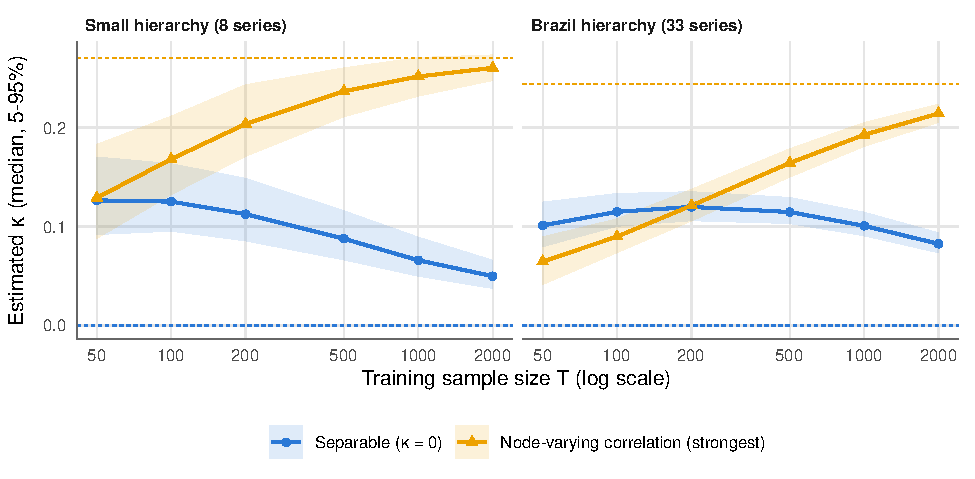
\includegraphics[width=\textwidth]{Imagens/kappa_noise.pdf}
  \caption{Sampling distribution of $\widehat\kappa$ (median and 5--95\% range over 1000 replications) under a separable covariance and under the strongest node-varying correlation case, with the population values dashed.}
  \label{fig:noise}
\end{figure}

We calibrate them with a parametric bootstrap that reproduces the estimation step:
\begin{enumerate}
  \item Estimate $\widehat{\bm{W}}$ from the $T$ residual vectors, and compute $\widehat\kappa$ and $\widehat\gamma$.
  \item Form the null covariance $\bm{W}_0$, the nearest Kronecker approximation to $\widehat{\bm{W}}$, which satisfies Proposition~\ref{prop:equivalence}.
  \item For $b = 1,\dots,B$, simulate $T$ vectors from $N(\bm{0}, \bm{W}_0)$, re-estimate the covariance with the same estimator, and compute $\kappa_b$ and $\gamma_b$.
  \item Report $p$-values $(1 + \#\{\kappa_b \ge \widehat\kappa\})/(B+1)$ and similarly for $\gamma$.
\end{enumerate}
The null covariance is one member of the set on which $\kappa = \gamma = 0$. It is the natural choice because it is the separable matrix closest to the data, but other members of the null set would give somewhat different null distributions. Figure~\ref{fig:power} reports the size and power of both tests for the covariance families of Section~\ref{sec:simulation}. \todo{summarise size and power, from power results}

\begin{figure}[!htb]
  \centering
  \includegraphics[width=\textwidth]{Imagens/gain_power.pdf}
  \caption{Rejection rate at the 5\% level of the bootstrap test based on $\widehat\gamma$ ($B = 199$, 200 replications), by sample size.}
  \label{fig:power}
\end{figure}
